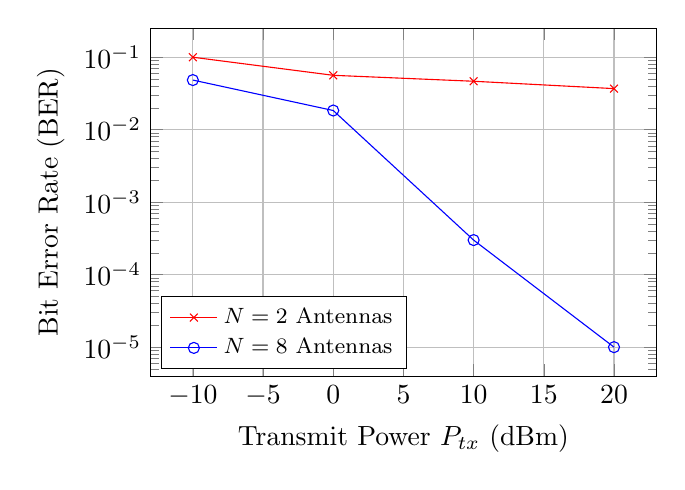
\begin{tikzpicture}
\begin{semilogyaxis}[
    xlabel={Transmit Power $P_{tx}$ (dBm)},
    ylabel={Bit Error Rate (BER)},
    grid=major,
    legend style={at={(0.02,0.02)}, anchor=south west, font=\footnotesize},
    width=8cm,
    height=6cm
]

% N=2
\addplot[color=red, mark=x] coordinates {
    (-10, 0.1000) (0, 0.0563) (10, 0.0466) (20, 0.0369)
};
\addlegendentry{$N=2$ Antennas}

% N=8
\addplot[color=blue, mark=o] coordinates {
    (-10, 0.0484) (0, 0.0184) (10, 0.0003) (20, 0.00001)
};
\addlegendentry{$N=8$ Antennas}

\end{semilogyaxis}
\end{tikzpicture}